% STATUS: ACTIVE -- c-only slope law with the wall position w_s as a constant state: model, estimator, error dynamics, Q and R,
%   and the single-seed results on the plane and cell walls next to c-only.
% ======================================================
% Compile: xelatex 1009_conly_wall_position.tex   (from reference/eq17_analysis/derivation/)
% Layout (user 2026-10-11): derivation and its result figures only, in the motion_ctrl_share.pdf convention (equations, section
%   titles, one setting line per figure page, no readings; preamble and \figpage copied from motion_ctrl.tex). Section 1 =
%   motion_ctrl/sec5_conly.tex with one state added; Section 2 = the constant-velocity descent of ramp_tri (22.2 -> 1.10 R in 1 s,
%   then parked 0.2 s; user 10-11: judge on the descent only), columns plane | cell; the c and w_s estimator only (no c-only column).
%   The walls page and the two fixed-height figures were removed (user 10-11); their runs stay in run_1009_ws.m (fixtop / fixbot).
%   The observability matrix and "what it shows" sections of the 10-09 version are set aside in archive/1009_conly_wall_position_v1.tex.
% Setting: c-only of motion_ctrl Section 6 unchanged (slope (1-c)/h^2, q55 = P_fix^2 I, sqrt(P_fix) 0.15, c-hat[0] = 0,
%   sqrt(p55[0]) 0.10, lambda_c 0.4) plus w_s: w_s-hat[0] = 0 (plane init, .claude/rules/wall-test-protocol.md), q66 = 0,
%   sqrt(p66[0]) = 0.64 (run_plaw_walls f2 default = half the wall-family spread of delta; not derived, open).
%   Red lines: c(h_d) = 1 - h_d^2 a'(h_d) of the wall and w_s = 0, the wall position set in the plant (both walls touch at h = 1).
% Code: formC_b. c-only = run_plaw_walls law 'f1p2' ctrl_const (plaw_cp_slope, slot 7 = p pinned at 2); with w_s = law 'f2'
%   ctrl_const (plaw_dc_slope, slope (1-c)/(h + delta)^2, slot 7 = delta = -w_s, clamp delta in [-0.9, 3], gap floor 0.5),
%   delta-hat[0] = 0. Slot 7 has no Q entry (Q_i only fills 3-4 and q55). The code walks y2 back d steps; the text writes the
%   delay-free H as motion_ctrl S5 (C92).
% Runs: test_script/scratch/run_1009_ws.m (scen fixtop / fixbot / desc, arm 'ws', seed 1; test_results/temp_1009_ws).
%   Figures: plot_1009_ws.m (prints e_a, c-hat, w_s-hat, sqrt(P), accumulated information on c, slope ratio of the end pair).
%   Fig. 2.2 (user 10-11: window = 3 steps so O is square; focus v4, v5, v6; no red formula line for now): probe_1009_ws_svd3_track.m
%   (obs_dump capture of the Fig. 2.1 run, O(k) from the code's F_e, H, R at every k; the computation divides each row by sqrt(r),
%   the text shows O without R (user 10-11: R not in the text for now, results unchanged); the code's H walks y2 back d steps, the text's H
%   does not, C92), figure plot_1009_ws_svd3.m. Checks: max |V'V - I| 1.6e-15; dx1..3 components of v4..v6 <= 7e-5 (so only the
%   a, c, w_s components are drawn); v6 c : w_s vs 2(1 - c-hat)/(h_d - w_s-hat) median relative difference 0.3-0.4 % (not drawn).
%   sigma_1..3 = 1/sqrt(r1) = 680 (dx1..3 through y1, not drawn). Explanation figure (conversation only): plot_1009_ws_v56_meaning.m.
%   Window notation (10-12): O(k0, k1) = rows H Phi(j, k0), j = k0..k1; 3-step window O(k0, k0+2) (Fig. 2.2), window from the start
%   O(0, k) (Fig. 2.3, probe_1009_ws_svd_cum.m: G = O'O accumulated step by step, rows / sqrt(r) as Fig. 2.2; vectors picked by content,
%   the a-direction becomes the largest sigma once y2 accumulates; where it crosses the dx sigmas 680 (~0.28 s) the most a-like vector of
%   the equal-sigma group is drawn, user 10-12). The which-window figure (plot_1009_ws_which_window.m, bounds sqrt([(P0^-1 + O'O)^-1]_ww),
%   no Q) was removed from the text (user 10-12); its readings stay below.
%   Measured 10-12 (seed 1): O(0,k) beats the prior along v6 at t = 0.748 s (6.4 R, plane) / 0.760 s (6.2 R, cell), where w_s-hat
%   starts to fall; sqrt(p66) at the end 0.096 / 0.295 vs O(0,k) bound 0.011 / 0.049 (no Q), O(k0,k0+2) bound 0.640; cell estimator
%   long axis dc/dw_s 0.446 vs O(0,k) v6 0.423. O(0,k) at the end: sigma_5 / sigma_6 = 536 / 65 (plane), 196 / 14.4 (cell).
%   Instrument checks (10-11, scen tri10): the c-only arm reproduces the cached motion_ctrl Fig. 6.3 / 6.4 runs bit for bit;
%   the w_s arm with sqrt(p66[0]) = 1e-6 lands on c-only (max |d a-hat| 1.3e-11, |d c-hat| 1.9e-10).
% Measured 10-11 (seed 1, e_a = a_true - a_hat):
%   top    : c-hat +0.02, w_s-hat -0.03, sqrt(P) 0.10 / 0.64 unchanged, |e_a| <= 0.003 (both walls).
%   bottom : plane c-hat -0.05, w_s-hat +0.12 (sqrt(P_w) 0.09); cell c-hat +0.01, w_s-hat -0.58 (0.11), a-hat jumps to 0.95 in the
%            first 10 ms and is 0.66 at 2 s (true 0.505; c-only 0.64). Seed cross terms off: plane w_s-hat -0.50, cell +0.64 (sqrt(P_w) 0.04).
%   descent: plane end pair (-0.03, -0.05), slope ratio 1.00 / 1.00 / 0.93 at h = 1.1 / 2 / 5; cell (+0.04, -1.00), 1.02 / 0.96 / 0.89;
%            w_s-hat leaves its prior only below ~6 R (sqrt(P_w) 0.64 -> 0.54 at 6.4 R, 0.43 at 3.2 R, 0.28-0.30 at 1.10 R on the cell);
%            descent |e_a| mean 0.012 / 0.015, worst 0.073 / 0.057 (plane / cell).
% Section 3 (user 10-12): c-only (motion_ctrl S6, unchanged) with the plant's plane wall at w_s = DELTA; the plant handle feeds the
%   mobility (calc_gamma_inv) and the thermal force (calc_thermal_force), the estimator keeps w_s = 0. Runs run_1009_wallshift.m
%   (DELTA 0, -2, -4, +2, +4; 10 seeds; red c = the wall's own c at the true gap g = h_true - DELTA, user 10-13; check DELTA = 0 handle vs production 5e-16), figures plot_1009_wallshift.m ('neg', 'pos'; sqrt(P_fix) 0.15 everywhere,
%   user 10-12). A per-case sqrt(P_fix) sweep (probe_1009_wallshift_pfix.m, reference arm) exists but is not in the text; 'law' = offline curves.
% Section 4 (user 10-13): the c-only law with the numerator fixed at 1, the wall position w_s estimated instead of c, q55 = 0
%   (w_s constant). Code: formC_b plaw_dc_slope with c pinned (c_init 0, Pf_c_std ~ 0, no q55 on c), slot 7 = delta = -w_s;
%   widen plaw_delta_lim (default [-0.9, 3] = w_s in [-3, 0.9]). Derivation only so far; no run yet.
% Check: python3 test_script/scratch/check_1009_conly_wall_position.py (sympy; row 4 of F_e is part (1)-(2) of it).
% ======================================================
\documentclass[11pt,a4paper]{ctexart}
\usepackage[fleqn]{amsmath}
\usepackage{amssymb,bm}
\usepackage{graphicx}
\graphicspath{{figures/}}
\setlength{\mathindent}{0pt}
\usepackage{geometry}
\geometry{margin=2.2cm}
\setlength{\parindent}{0pt}
\setlength{\parskip}{0.2em}
\setlength{\abovedisplayskip}{6pt}
\setlength{\belowdisplayskip}{6pt}
\setlength{\abovedisplayshortskip}{6pt}
\setlength{\belowdisplayshortskip}{6pt}
\newcommand{\lc}{\lambda_c}
\newcommand{\bx}{\bar{x}}
\newcommand{\ba}{\bar{a}}
\newcommand{\bw}{\bar{w}}
\newcommand{\hh}{\hat{h}}
\newcommand{\ch}{\hat{c}}
\newcommand{\hd}[1]{\par\bigskip\noindent\underline{\textbf{#1}}}
% one figure page: title, one setting line, the figure
\newcommand{\figpage}[3]{\clearpage\subsection*{#1}\noindent{\small\textcolor[gray]{0.35}{#2}}\par\smallskip
  \begin{center}\includegraphics[width=\textwidth,height=0.82\textheight,keepaspectratio]{#3}\end{center}}
\usepackage{xcolor}
\pagestyle{plain}

\begin{document}

\begin{center}
{\Large\textbf{Position-dependent motion gain with an unknown wall position}}
\end{center}

%======================================================================
\section{Real-time estimation with the wall position as a state}

\hd{Motion gain as a function of the distance from the wall}
\[
\begin{aligned}
h[k] &= \bx_d[k] - \delta\bx_3[k] - \bw_s \\
\ba'[k] &= \frac{1 - c}{h[k]^{2}} \\
M[k] &= \Delta\bx_d[k] + (1-\lc)\,\delta\bx_3[k]
\end{aligned}
\]

\hd{State of the process}
\[
\begin{aligned}
\delta\bx_1[k+1] &= \delta\bx_2[k] \\
\delta\bx_2[k+1] &= \delta\bx_3[k] \\
\delta\bx_3[k+1] &= \lc\,\delta\bx_3[k] - F_{dx}[k]\,e_{\ba}[k] - \varepsilon_x[k] \\
\ba[k+1] &= \ba[k] + \ba'[k]\,\big(M[k] + F_{dx}[k]\,e_{\ba}[k] + \varepsilon_x[k]\big) \\
c[k+1] &= c[k] \\
\bw_s[k+1] &= \bw_s[k]
\end{aligned}
\]

\hd{Measurement and output matrix}
\[
\mathbf{y}[k] = \begin{bmatrix} \delta\bx_m[k] \\ \ba_m[k] \end{bmatrix},
\qquad
\hat{\mathbf{y}}[k] = \begin{bmatrix} \delta\hat{\bx}_1[k] \\ \hat{\ba}[k] \end{bmatrix},
\qquad
\mathbf{H} =
\begin{bmatrix}
1 & 0 & 0 & 0 & 0 & 0 \\
0 & 0 & 0 & 1 & 0 & 0
\end{bmatrix}
\]

\hd{Estimator}
\[
\begin{aligned}
\hh[k] &= \bx_d[k] - \delta\hat{\bx}_3[k] - \hat{\bw}_s[k] \\
\hat{\ba}'[k] &= \frac{1 - \ch[k]}{\hh[k]^{2}} \\
\hat{M}[k] &= \Delta\bx_d[k] + (1-\lc)\,\delta\hat{\bx}_3[k]
\end{aligned}
\]
\[
\begin{aligned}
\delta\hat{\bx}_1[k+1] &= \delta\hat{\bx}_2[k] + \big\{\ell_{11}[k]\,e_{x_1}[k] + \ell_{12}[k]\,e_{a_m}[k]\big\} \\
\delta\hat{\bx}_2[k+1] &= \delta\hat{\bx}_3[k] + \big\{\ell_{21}[k]\,e_{x_1}[k] + \ell_{22}[k]\,e_{a_m}[k]\big\} \\
\delta\hat{\bx}_3[k+1] &= \lc\,\delta\hat{\bx}_3[k] + \big\{\ell_{31}[k]\,e_{x_1}[k] + \ell_{32}[k]\,e_{a_m}[k]\big\} \\
\hat{\ba}[k+1] &= \hat{\ba}[k] + \hat{\ba}'[k]\,\hat{M}[k] + \big\{\ell_{41}[k]\,e_{x_1}[k] + \ell_{42}[k]\,e_{a_m}[k]\big\} \\
\ch[k+1] &= \ch[k] + \big\{\ell_{51}[k]\,e_{x_1}[k] + \ell_{52}[k]\,e_{a_m}[k]\big\} \\
\hat{\bw}_s[k+1] &= \hat{\bw}_s[k] + \big\{\ell_{61}[k]\,e_{x_1}[k] + \ell_{62}[k]\,e_{a_m}[k]\big\}
\end{aligned}
\]

\hd{Dynamics of estimation errors}
\[
\mathbf{e}[k] = \begin{bmatrix} e_{\delta\bx_1}[k] \\ e_{\delta\bx_2}[k] \\ e_{\delta\bx_3}[k] \\ e_{\ba}[k] \\ e_c[k] \\ e_{\bw_s}[k] \end{bmatrix},
\qquad
\mathbf{e}[k+1] = \mathbf{F}_e[k]\,\mathbf{e}[k] - \mathbf{L}[k]\,\mathbf{H}\,\mathbf{e}[k] + \mathbf{q}[k]
\]
{\small
\[
\mathbf{F}_e[k] =
\begin{bmatrix}
0 & 1 & 0 & 0 & 0 & 0 \\
0 & 0 & 1 & 0 & 0 & 0 \\
0 & 0 & \lc & -F_{dx}[k] & 0 & 0 \\
0 & 0 & \;\hat{\ba}'[k]\,(1-\lc) + \dfrac{2\,\hat{\ba}'[k]}{\hh[k]}\,\hat{M}[k]\; & 1 + \hat{\ba}'[k]\,F_{dx}[k] & -\dfrac{\hat{M}[k]}{\hh[k]^{2}} & \dfrac{2\,\hat{\ba}'[k]}{\hh[k]}\,\hat{M}[k] \\
0 & 0 & 0 & 0 & 1 & 0 \\
0 & 0 & 0 & 0 & 0 & 1
\end{bmatrix}
\]
}
\[
\mathbf{q}[k] = \begin{bmatrix} 0 \\ 0 \\ -\varepsilon_x[k] \\ \hat{\ba}'[k]\,\varepsilon_x[k] \\ 0 \\ 0 \end{bmatrix}
\]

\clearpage
\hd{Row 4 of $\mathbf{F}_e$, expanded}

\noindent (a) the two gain steps and their difference
\[
\begin{aligned}
\ba[k+1] - \ba[k] &= \ba'[k]\,\big(M[k] + F_{dx}[k]\,e_{\ba}[k] + \varepsilon_x[k]\big) \\
\hat{\ba}[k+1] - \hat{\ba}[k] &= \hat{\ba}'[k]\,\hat{M}[k] \\
e_{\ba}[k+1] - e_{\ba}[k] &= \ba'[k]\,M[k] - \hat{\ba}'[k]\,\hat{M}[k] + \ba'[k]\,F_{dx}[k]\,e_{\ba}[k] + \ba'[k]\,\varepsilon_x[k]
\end{aligned}
\]

\noindent (b) each factor written as its estimate plus its error
\[
\begin{aligned}
h[k] &= \hh[k] - e_{\delta\bx_3}[k] - e_{\bw_s}[k], \qquad c = \ch[k] + e_c[k] \\
\ba'[k] &= \frac{1 - \ch[k] - e_c[k]}{\big(\hh[k] - e_{\delta\bx_3}[k] - e_{\bw_s}[k]\big)^{2}}
= \hat{\ba}'[k] + \frac{2\,\hat{\ba}'[k]}{\hh[k]}\,\big(e_{\delta\bx_3}[k] + e_{\bw_s}[k]\big) - \frac{1}{\hh[k]^{2}}\,e_c[k] + O(e^{2}) \\
M[k] &= \hat{M}[k] + (1-\lc)\,e_{\delta\bx_3}[k]
\end{aligned}
\]

\noindent (c) the product difference, exact
\[
\ba'[k]\,M[k] - \hat{\ba}'[k]\,\hat{M}[k]
= \hat{\ba}'[k]\,\big(M[k] - \hat{M}[k]\big) + \big(\ba'[k] - \hat{\ba}'[k]\big)\,\hat{M}[k] + \big(\ba'[k] - \hat{\ba}'[k]\big)\big(M[k] - \hat{M}[k]\big)
\]

\noindent (d) every term after substituting (b)
\[
\begin{aligned}
e_{\ba}[k+1] - e_{\ba}[k]
&= \hat{\ba}'[k]\,(1-\lc)\,e_{\delta\bx_3}[k] \\
&\quad + \frac{2\,\hat{\ba}'[k]}{\hh[k]}\,\hat{M}[k]\,e_{\delta\bx_3}[k] - \frac{\hat{M}[k]}{\hh[k]^{2}}\,e_c[k] + \frac{2\,\hat{\ba}'[k]}{\hh[k]}\,\hat{M}[k]\,e_{\bw_s}[k] \\
&\quad + \hat{\ba}'[k]\,F_{dx}[k]\,e_{\ba}[k] + \hat{\ba}'[k]\,\varepsilon_x[k] \\
&\quad + \Big(\frac{2\,\hat{\ba}'[k]}{\hh[k]}\,\big(e_{\delta\bx_3}[k] + e_{\bw_s}[k]\big) - \frac{e_c[k]}{\hh[k]^{2}}\Big) \\
&\qquad\quad \times\Big((1-\lc)\,e_{\delta\bx_3}[k] + F_{dx}[k]\,e_{\ba}[k] + \varepsilon_x[k]\Big) + O(e^{2})
\end{aligned}
\]

\noindent (e) first-order terms collected by error
\[
\begin{aligned}
e_{\ba}[k+1] &= \Big(\hat{\ba}'[k]\,(1-\lc) + \frac{2\,\hat{\ba}'[k]}{\hh[k]}\,\hat{M}[k]\Big)\,e_{\delta\bx_3}[k] \\
&\quad + \big(1 + \hat{\ba}'[k]\,F_{dx}[k]\big)\,e_{\ba}[k] \\
&\quad - \frac{\hat{M}[k]}{\hh[k]^{2}}\,e_c[k] \\
&\quad + \frac{2\,\hat{\ba}'[k]}{\hh[k]}\,\hat{M}[k]\,e_{\bw_s}[k] \\
&\quad + \hat{\ba}'[k]\,\varepsilon_x[k]
\end{aligned}
\]

\hd{Process noise and measurement noise}
\[
\begin{aligned}
\mathbf{Q}[k] &=
\begin{bmatrix}
0 & 0 & 0 & 0 & 0 & 0 \\
0 & 0 & 0 & 0 & 0 & 0 \\
0 & 0 & q_{33}[k] & -\hat{\ba}'[k]\,q_{33}[k] & 0 & 0 \\
0 & 0 & -\hat{\ba}'[k]\,q_{33}[k] & \hat{\ba}'[k]^{2}\,q_{33}[k] & 0 & 0 \\
0 & 0 & 0 & 0 & q_{55}[k] & 0 \\
0 & 0 & 0 & 0 & 0 & q_{66}
\end{bmatrix} \\
q_{55}[k] &= P_{\mathrm{fix}}^{2}\, I[k], \qquad I[k] = \frac{1}{p_{55}[k]} - \frac{1}{p^f_{55}[k]} \\
q_{66} &= 0 \\
\mathbf{R}[k] &= \mathrm{diag}\big(r_1,\ r_2[k]\big)
\end{aligned}
\]
($q_{33}$, $r_1$, $r_2$, $\mathbf{L}$, $\mathbf{P}$, $\mathbf{P}^f$ as in motion\_ctrl Section 4; $q_{55}$ as in motion\_ctrl Section 6.)

%======================================================================
\clearpage
\section{Constant-velocity descent}
\subsection*{Fig.~2.1\quad Descent 22.2 $\to$ 1.10 R}
\noindent{\small\textcolor[gray]{0.35}{z axis; 22.2 $\to$ 1.10 R at constant velocity in 1 s, then parked at 1.10 R for 0.2 s; left: plane wall; right: cell wall; red: $c(h_d) = 1 - h_d^{2}\,\ba'(h_d)$ and $\bw_s = 0$; $\sqrt{P_{\mathrm{fix}}} = 0.15$, $q_{66} = 0$, $\ch[0] = 0$, $\hat{\bw}_s[0] = 0$, $\sqrt{p_{66}[0]} = 0.64$; $\lc = 0.4$, seed 1}}\par\smallskip
\begin{center}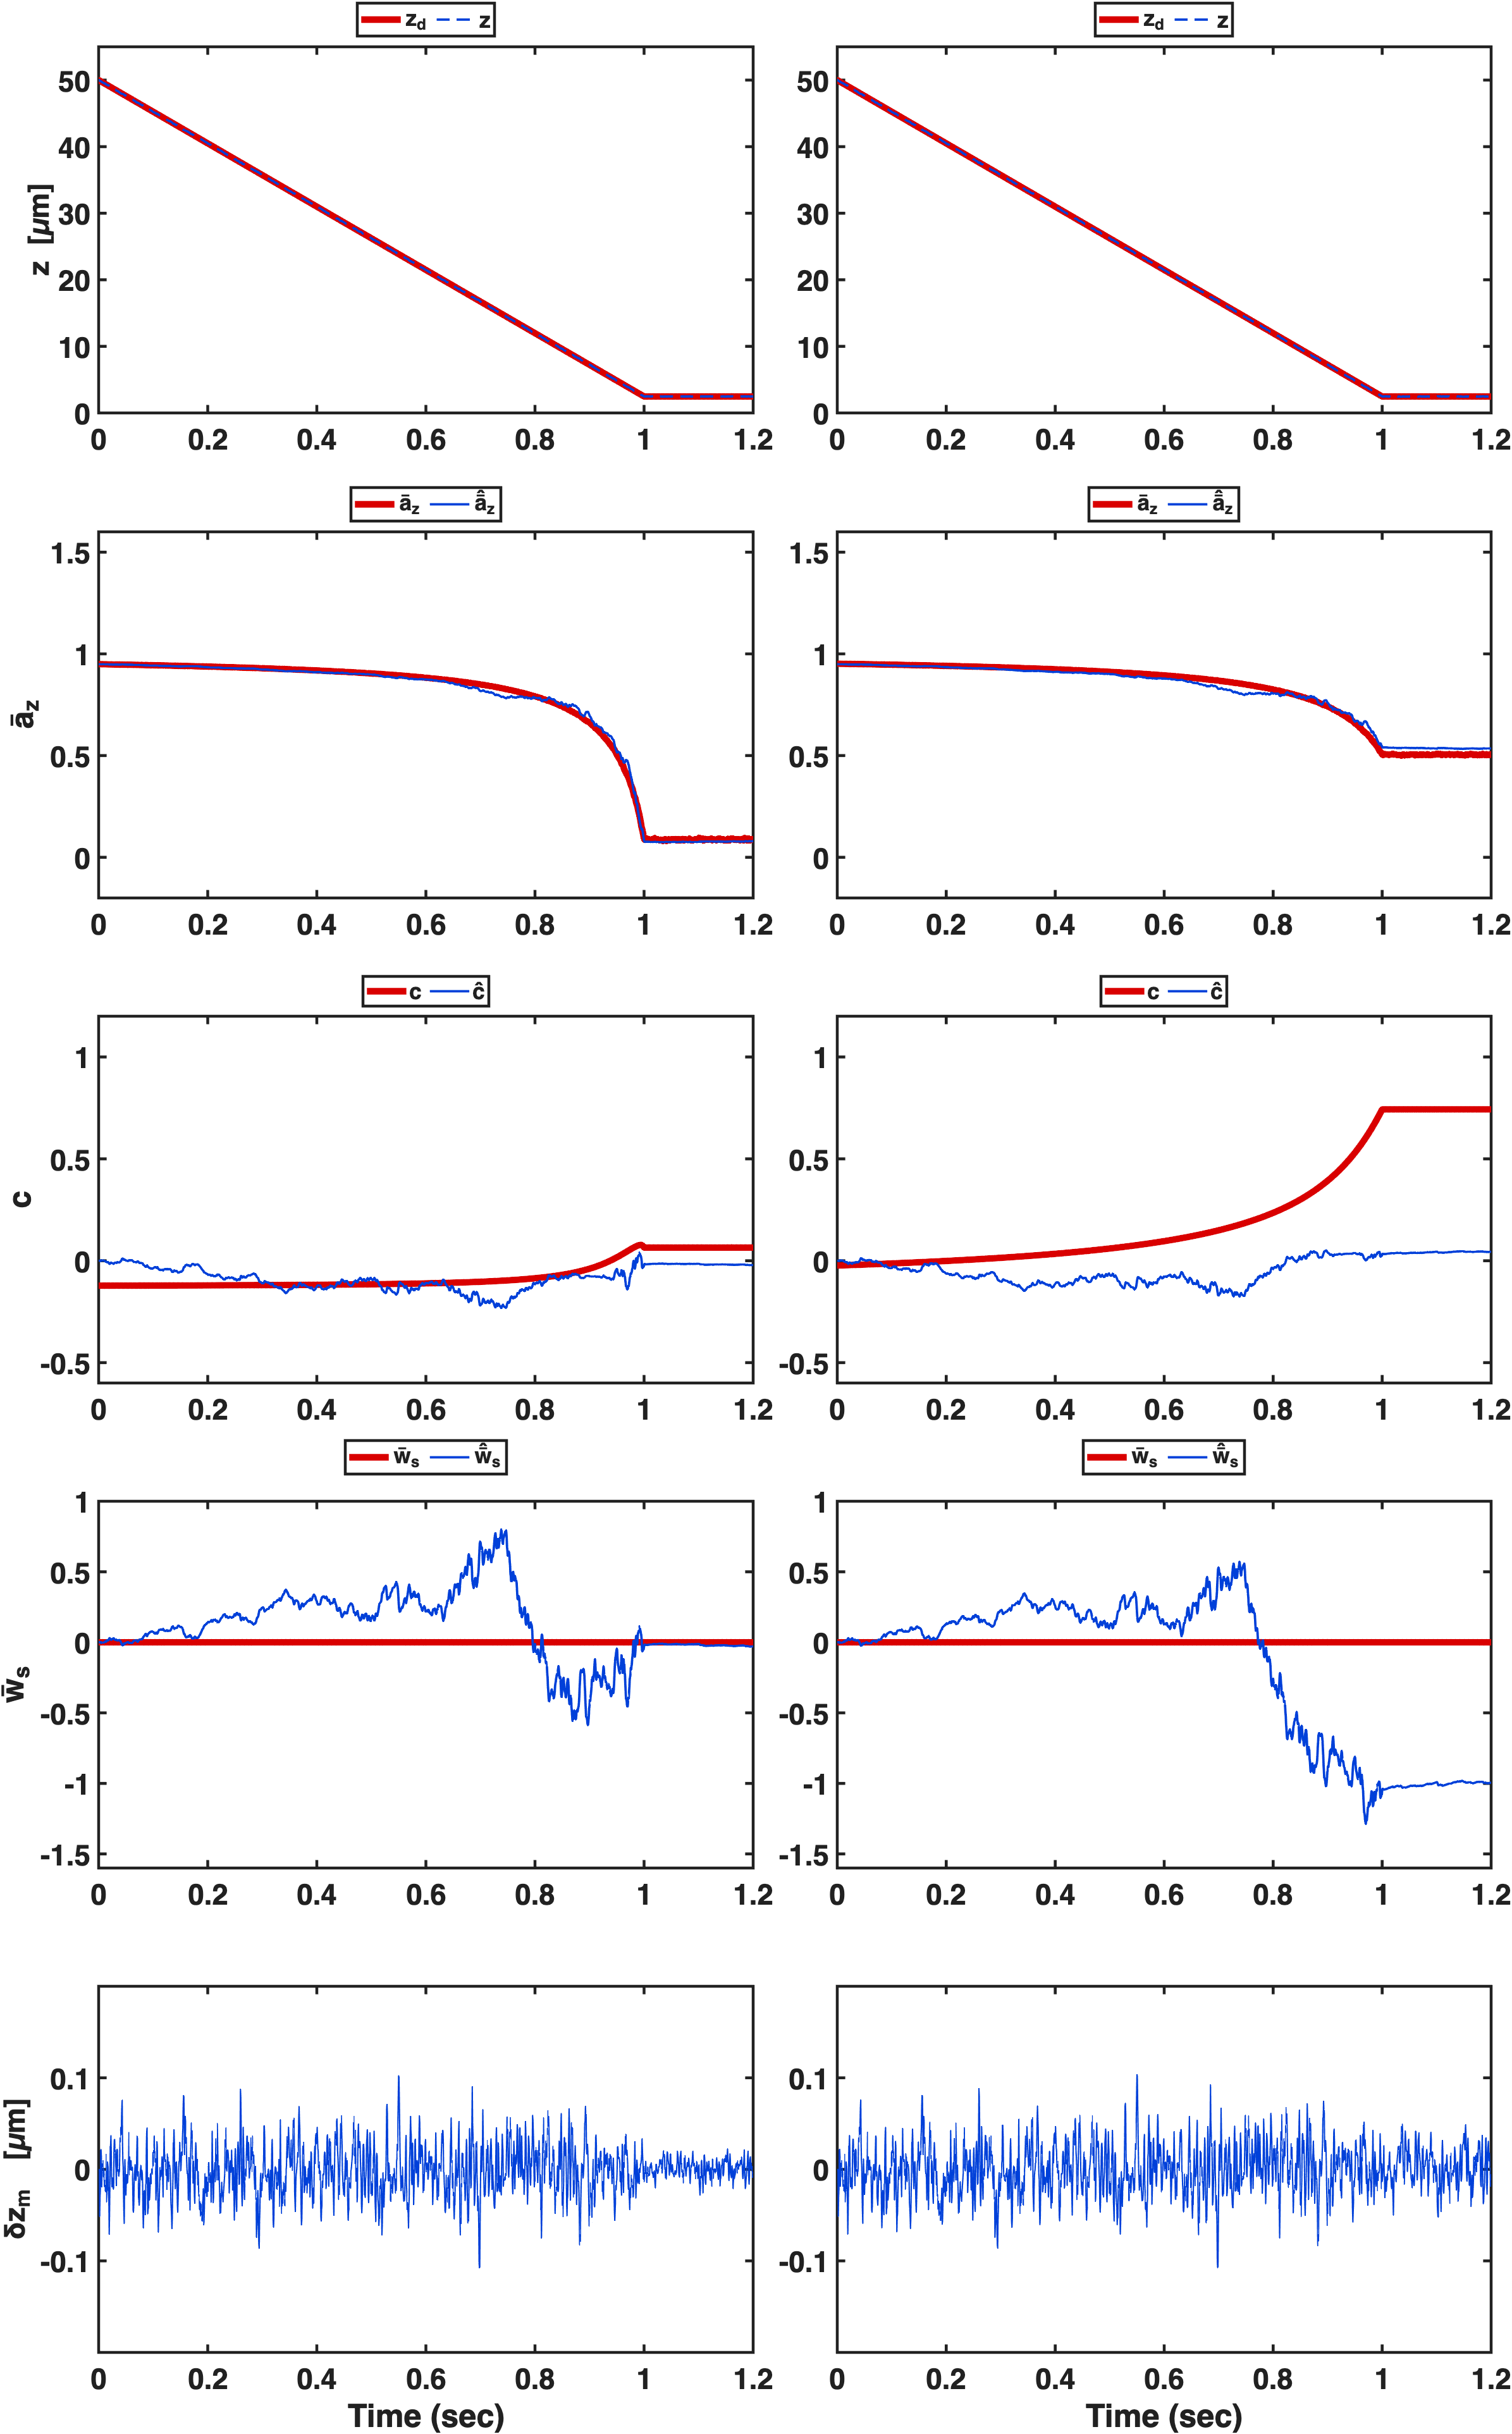
\includegraphics[width=\textwidth,height=0.82\textheight,keepaspectratio]{fig_1009_ws_desc_s1.png}\end{center}

\clearpage
\hd{Error propagation (no noise, coefficients at the estimate)}
\[
\begin{aligned}
\mathbf{e}[k+1] &= \mathbf{F}_e[k]\,\mathbf{e}[k] \\
\mathbf{e}[k_0+j] &= \bm{\Phi}(k_0+j,k_0)\,\mathbf{e}[k_0], \qquad
\bm{\Phi}(k_0+j,k_0) = \mathbf{F}_e[k_0+j-1]\cdots\mathbf{F}_e[k_0], \qquad
\bm{\Phi}(k_0,k_0) = \mathbf{I}
\end{aligned}
\]

\hd{Errors at step $k_0$, output errors $j$ steps later}
\[
\begin{bmatrix} e_{x_1}[k_0+j] \\ e_{a_m}[k_0+j] \end{bmatrix}
= \mathbf{H}\,\bm{\Phi}(k_0+j,k_0)\,\mathbf{e}[k_0]
\]

\hd{Observability matrix from step $k_0$ to step $k_1$}
\[
\begin{bmatrix}
e_{x_1}[k_0] \\ e_{a_m}[k_0] \\[0.4ex]
e_{x_1}[k_0+1] \\ e_{a_m}[k_0+1] \\[0.4ex]
\vdots \\[0.4ex]
e_{x_1}[k_1] \\ e_{a_m}[k_1]
\end{bmatrix}
=
\underbrace{\begin{bmatrix}
\mathbf{H} \\[0.4ex]
\mathbf{H}\,\bm{\Phi}(k_0+1,k_0) \\[0.4ex]
\vdots \\[0.4ex]
\mathbf{H}\,\bm{\Phi}(k_1,k_0)
\end{bmatrix}}_{\mathbf{O}(k_0,\,k_1)}
\begin{bmatrix} e_{\delta\bx_1}[k_0] \\ e_{\delta\bx_2}[k_0] \\ e_{\delta\bx_3}[k_0] \\ e_{\ba}[k_0] \\ e_c[k_0] \\ e_{\bw_s}[k_0] \end{bmatrix}
\]

\hd{Window of three steps ($6 \times 6$): $k_1 = k_0 + 2$, the window moves one step at a time}
\[
\mathbf{O}(k_0,\,k_0+2) =
\begin{bmatrix}
\mathbf{H} \\[0.4ex]
\mathbf{H}\,\mathbf{F}_e[k_0] \\[0.4ex]
\mathbf{H}\,\mathbf{F}_e[k_0+1]\,\mathbf{F}_e[k_0]
\end{bmatrix},
\qquad
\mathbf{O}(k_0+1,\,k_0+3) =
\begin{bmatrix}
\mathbf{H} \\[0.4ex]
\mathbf{H}\,\mathbf{F}_e[k_0+1] \\[0.4ex]
\mathbf{H}\,\mathbf{F}_e[k_0+2]\,\mathbf{F}_e[k_0+1]
\end{bmatrix}
\]

\hd{Window from the start of the descent: $k_0 = 0$, the window grows one step at a time}
\[
\mathbf{O}(0,\,k) =
\begin{bmatrix}
\mathbf{H} \\[0.4ex]
\mathbf{H}\,\bm{\Phi}(1,0) \\[0.4ex]
\vdots \\[0.4ex]
\mathbf{H}\,\bm{\Phi}(k,0)
\end{bmatrix},
\qquad
\mathbf{O}(0,\,k+1) =
\begin{bmatrix}
\mathbf{O}(0,\,k) \\[0.4ex]
\mathbf{H}\,\bm{\Phi}(k+1,0)
\end{bmatrix},
\qquad
\bm{\Phi}(k+1,0) = \mathbf{F}_e[k]\,\bm{\Phi}(k,0)
\]

\figpage{Fig.~2.2\quad Three-step window $\mathbf{O}(k_0,\,k_0+2)$ along the descent: $\sigma_4$, $\sigma_5$, $\sigma_6$ and $\mathbf{v}_4$, $\mathbf{v}_5$, $\mathbf{v}_6$}{z axis; run of Fig.~2.1; one window at every step $k_0$, plotted at $t = k_0 T_s$; $\sigma_i$, $\mathbf{v}_i$ = singular values and right singular vectors of $\mathbf{O}(k_0,\,k_0+2)$; rows: $h_d$, $\sigma_4$--$\sigma_6$, the $\ba$, $c$, $\bw_s$ components of $\mathbf{v}_4$, $\mathbf{v}_5$, $\mathbf{v}_6$ (sign of each $\mathbf{v}_i$ fixed by a positive $v_{4,\ba}$, $v_{5,c}$, $v_{6,\bw_s}$); left: plane wall; right: cell wall; seed 1}{fig_1009_ws_svd3_desc_s1.png}
\figpage{Fig.~2.3\quad Window from the start $\mathbf{O}(0,\,k)$ along the descent: $\sigma$ and $\mathbf{v}$ of $\ba$, $\sigma_5$, $\sigma_6$, $\mathbf{v}_5$, $\mathbf{v}_6$}{z axis; run of Fig.~2.1; $\mathbf{O}(0,\,k)$ at every step $k$, plotted at $t = k T_s$; $\mathbf{v}(\ba)$ = the right singular vector with the largest $\ba$ component (the largest $\sigma$ once the $\ba_m$ readings accumulate), $\mathbf{v}_5$, $\mathbf{v}_6$ = the two with the largest $c$, $\bw_s$ components; rows: $h_d$, the three $\sigma$, the $\ba$, $c$, $\bw_s$ components of $\mathbf{v}(\ba)$, $\mathbf{v}_5$, $\mathbf{v}_6$; left: plane wall; right: cell wall; seed 1}{fig_1009_ws_svdcum_desc_s1.png}

%======================================================================
\clearpage
\section{c-only with a wall-position error}

\hd{Wall of the plant at $\bw_s = \Delta$ (plane wall; plant only)}
\[
\begin{aligned}
D_\perp(u) &= 1 - \tfrac{9}{8}\,u + \tfrac{1}{2}\,u^{3} - \tfrac{57}{100}\,u^{4} + \tfrac{1}{5}\,u^{5} + \tfrac{7}{200}\,u^{11} - \tfrac{1}{25}\,u^{12} \\
\ba_{\mathrm{plant}}(h) &= D_\perp\Big(\frac{1}{h - \Delta}\Big)
\end{aligned}
\]

\hd{Estimator (motion\_ctrl Section 6, unchanged: wall at $\bw_s = 0$)}
\[
\begin{aligned}
\hh[k] &= \bx_d[k] - \delta\hat{\bx}_3[k] \\
\hat{\ba}'[k] &= \frac{1 - \ch[k]}{\hh[k]^{2}} \\
q_{55}[k] &= P_{\mathrm{fix}}^{2}\, I[k]
\end{aligned}
\]

\hd{Value of $c$ of the wall at the true gap $g = h - \Delta$}
\[
\ba_{\mathrm{plant}}'(h) = \frac{1 - c(g)}{g^{2}} \quad\Longrightarrow\quad c(g) = 1 - g^{2}\,\ba_{\mathrm{plant}}'(h), \qquad g = h - \Delta
\]

\hd{Trajectory}
\[
h_d:\ 22.2 \;\to\; 1.10 + \max(\Delta, 0) \ \text{ in } 1\ \mathrm{s}, \quad \text{then hold } 0.2\ \mathrm{s}
\]

\figpage{Fig.~3.1\quad Wall farther than assumed: $\Delta = 0,\ -2,\ -4$ R}{z axis; c-only of motion\_ctrl Section 6, $\sqrt{P_{\mathrm{fix}}} = 0.15$ in every case; red in the $c$ row: $c(g)$ at the true gap of the particle, dotted: numerical clamp of $\ch$, $[-3, 1]$; $\ch[0] = 0$, $\lc = 0.4$, seed 1}{fig_1009_wallshift_neg_s1.png}
\figpage{Fig.~3.2\quad Wall closer than assumed: $\Delta = 0,\ +2,\ +4$ R}{z axis; bottom $h_d = 1.10 + \Delta$ (true gap 1.10); c-only of motion\_ctrl Section 6, $\sqrt{P_{\mathrm{fix}}} = 0.15$ in every case; red in the $c$ row: $c(g)$ at the true gap of the particle, dotted: numerical clamp of $\ch$, $[-3, 1]$; $\ch[0] = 0$, $\lc = 0.4$, seed 1}{fig_1009_wallshift_pos_s1.png}

%======================================================================
\clearpage
\section{Slope with unit numerator, the wall position as the state}

\hd{Motion gain as a function of the distance from the wall}
\[
\begin{aligned}
h[k] &= \bx_d[k] - \delta\bx_3[k] - \bw_s \\
\ba'[k] &= \frac{1}{h[k]^{2}} \\
M[k] &= \Delta\bx_d[k] + (1-\lc)\,\delta\bx_3[k]
\end{aligned}
\]

\hd{State of the process}
\[
\begin{aligned}
\delta\bx_1[k+1] &= \delta\bx_2[k] \\
\delta\bx_2[k+1] &= \delta\bx_3[k] \\
\delta\bx_3[k+1] &= \lc\,\delta\bx_3[k] - F_{dx}[k]\,e_{\ba}[k] - \varepsilon_x[k] \\
\ba[k+1] &= \ba[k] + \ba'[k]\,\big(M[k] + F_{dx}[k]\,e_{\ba}[k] + \varepsilon_x[k]\big) \\
\bw_s[k+1] &= \bw_s[k]
\end{aligned}
\]

\hd{Measurement and output matrix}
\[
\mathbf{y}[k] = \begin{bmatrix} \delta\bx_m[k] \\ \ba_m[k] \end{bmatrix},
\qquad
\hat{\mathbf{y}}[k] = \begin{bmatrix} \delta\hat{\bx}_1[k] \\ \hat{\ba}[k] \end{bmatrix},
\qquad
\mathbf{H} =
\begin{bmatrix}
1 & 0 & 0 & 0 & 0 \\
0 & 0 & 0 & 1 & 0
\end{bmatrix}
\]

\hd{Estimator}
\[
\begin{aligned}
\hh[k] &= \bx_d[k] - \delta\hat{\bx}_3[k] - \hat{\bw}_s[k] \\
\hat{\ba}'[k] &= \frac{1}{\hh[k]^{2}} \\
\hat{M}[k] &= \Delta\bx_d[k] + (1-\lc)\,\delta\hat{\bx}_3[k]
\end{aligned}
\]
\[
\begin{aligned}
\delta\hat{\bx}_1[k+1] &= \delta\hat{\bx}_2[k] + \big\{\ell_{11}[k]\,e_{x_1}[k] + \ell_{12}[k]\,e_{a_m}[k]\big\} \\
\delta\hat{\bx}_2[k+1] &= \delta\hat{\bx}_3[k] + \big\{\ell_{21}[k]\,e_{x_1}[k] + \ell_{22}[k]\,e_{a_m}[k]\big\} \\
\delta\hat{\bx}_3[k+1] &= \lc\,\delta\hat{\bx}_3[k] + \big\{\ell_{31}[k]\,e_{x_1}[k] + \ell_{32}[k]\,e_{a_m}[k]\big\} \\
\hat{\ba}[k+1] &= \hat{\ba}[k] + \hat{\ba}'[k]\,\hat{M}[k] + \big\{\ell_{41}[k]\,e_{x_1}[k] + \ell_{42}[k]\,e_{a_m}[k]\big\} \\
\hat{\bw}_s[k+1] &= \hat{\bw}_s[k] + \big\{\ell_{51}[k]\,e_{x_1}[k] + \ell_{52}[k]\,e_{a_m}[k]\big\}
\end{aligned}
\]

\hd{Dynamics of estimation errors}
\[
\mathbf{e}[k] = \begin{bmatrix} e_{\delta\bx_1}[k] \\ e_{\delta\bx_2}[k] \\ e_{\delta\bx_3}[k] \\ e_{\ba}[k] \\ e_{\bw_s}[k] \end{bmatrix},
\qquad
\mathbf{e}[k+1] = \mathbf{F}_e[k]\,\mathbf{e}[k] - \mathbf{L}[k]\,\mathbf{H}\,\mathbf{e}[k] + \mathbf{q}[k]
\]
\[
\mathbf{F}_e[k] =
\begin{bmatrix}
0 & 1 & 0 & 0 & 0 \\
0 & 0 & 1 & 0 & 0 \\
0 & 0 & \lc & -F_{dx}[k] & 0 \\
0 & 0 & \;\hat{\ba}'[k]\,(1-\lc) + \dfrac{2\,\hat{\ba}'[k]}{\hh[k]}\,\hat{M}[k]\; & 1 + \hat{\ba}'[k]\,F_{dx}[k] & \dfrac{2\,\hat{\ba}'[k]}{\hh[k]}\,\hat{M}[k] \\
0 & 0 & 0 & 0 & 1
\end{bmatrix},
\qquad
\mathbf{q}[k] = \begin{bmatrix} 0 \\ 0 \\ -\varepsilon_x[k] \\ \hat{\ba}'[k]\,\varepsilon_x[k] \\ 0 \end{bmatrix}
\]

\clearpage
\hd{Row 4 of $\mathbf{F}_e$, expanded}

\noindent (a) the two gain steps and their difference
\[
\begin{aligned}
\ba[k+1] - \ba[k] &= \ba'[k]\,\big(M[k] + F_{dx}[k]\,e_{\ba}[k] + \varepsilon_x[k]\big) \\
\hat{\ba}[k+1] - \hat{\ba}[k] &= \hat{\ba}'[k]\,\hat{M}[k] \\
e_{\ba}[k+1] - e_{\ba}[k] &= \ba'[k]\,M[k] - \hat{\ba}'[k]\,\hat{M}[k] + \ba'[k]\,F_{dx}[k]\,e_{\ba}[k] + \ba'[k]\,\varepsilon_x[k]
\end{aligned}
\]

\noindent (b) each factor written as its estimate plus its error
\[
\begin{aligned}
h[k] &= \hh[k] - e_{\delta\bx_3}[k] - e_{\bw_s}[k] \\
\ba'[k] &= \frac{1}{\big(\hh[k] - e_{\delta\bx_3}[k] - e_{\bw_s}[k]\big)^{2}}
= \hat{\ba}'[k] + \frac{2\,\hat{\ba}'[k]}{\hh[k]}\,\big(e_{\delta\bx_3}[k] + e_{\bw_s}[k]\big) + O(e^{2}) \\
M[k] &= \hat{M}[k] + (1-\lc)\,e_{\delta\bx_3}[k]
\end{aligned}
\]

\noindent (c) the product difference, exact
\[
\ba'[k]\,M[k] - \hat{\ba}'[k]\,\hat{M}[k]
= \hat{\ba}'[k]\,\big(M[k] - \hat{M}[k]\big) + \big(\ba'[k] - \hat{\ba}'[k]\big)\,\hat{M}[k] + \big(\ba'[k] - \hat{\ba}'[k]\big)\big(M[k] - \hat{M}[k]\big)
\]

\noindent (d) every term after substituting (b)
\[
\begin{aligned}
e_{\ba}[k+1] - e_{\ba}[k]
&= \hat{\ba}'[k]\,(1-\lc)\,e_{\delta\bx_3}[k] \\
&\quad + \frac{2\,\hat{\ba}'[k]}{\hh[k]}\,\hat{M}[k]\,e_{\delta\bx_3}[k] + \frac{2\,\hat{\ba}'[k]}{\hh[k]}\,\hat{M}[k]\,e_{\bw_s}[k] \\
&\quad + \hat{\ba}'[k]\,F_{dx}[k]\,e_{\ba}[k] + \hat{\ba}'[k]\,\varepsilon_x[k] \\
&\quad + \frac{2\,\hat{\ba}'[k]}{\hh[k]}\,\big(e_{\delta\bx_3}[k] + e_{\bw_s}[k]\big)\Big((1-\lc)\,e_{\delta\bx_3}[k] + F_{dx}[k]\,e_{\ba}[k] + \varepsilon_x[k]\Big) + O(e^{2})
\end{aligned}
\]

\noindent (e) first-order terms collected by error
\[
\begin{aligned}
e_{\ba}[k+1] &= \Big(\hat{\ba}'[k]\,(1-\lc) + \frac{2\,\hat{\ba}'[k]}{\hh[k]}\,\hat{M}[k]\Big)\,e_{\delta\bx_3}[k] \\
&\quad + \big(1 + \hat{\ba}'[k]\,F_{dx}[k]\big)\,e_{\ba}[k] \\
&\quad + \frac{2\,\hat{\ba}'[k]}{\hh[k]}\,\hat{M}[k]\,e_{\bw_s}[k] \\
&\quad + \hat{\ba}'[k]\,\varepsilon_x[k]
\end{aligned}
\]

\hd{Process noise and measurement noise}
\[
\begin{aligned}
\mathbf{Q}[k] &=
\begin{bmatrix}
0 & 0 & 0 & 0 & 0 \\
0 & 0 & 0 & 0 & 0 \\
0 & 0 & q_{33}[k] & -\hat{\ba}'[k]\,q_{33}[k] & 0 \\
0 & 0 & -\hat{\ba}'[k]\,q_{33}[k] & \hat{\ba}'[k]^{2}\,q_{33}[k] & 0 \\
0 & 0 & 0 & 0 & q_{55}
\end{bmatrix},
\qquad q_{55} = 0 \\
\mathbf{R}[k] &= \mathrm{diag}\big(r_1,\ r_2[k]\big)
\end{aligned}
\]
($q_{33}$, $r_1$, $r_2$, $\mathbf{L}$, $\mathbf{P}$, $\mathbf{P}^f$ as in motion\_ctrl Section 4.)

\end{document}
